% \documentclass[12pt]{article}

%%v helpful MIT exam schema, see http://www-math.mit.edu/~psh/exam/examdoc.pdf
 \documentclass[9pt]{exam} 
% \qformat{\textbf{Question \thequestion}\quad \thepoints\hfill } % Large depth to make space}
 \renewcommand{\thesubpart}{(\roman{subpart})}
 \renewcommand{\subpartlabel}{\thesubpart}
 \footer{}{}{Page \thepage\ de \numpages}
\addpoints
% \pointsinmargin
% \boxedpoints
%\renewcommand{\questionshook}{\setlength{\itemsep}{1cm}}
%\renewcommand{\partshook}{
%	\setlength{\itemsep}{0.5cm}
%    	\setlength{\leftmargin}{-10pt}%
%}

\usepackage{cmbright}

\pagestyle{empty} %for handouts
\addtolength{\jot}{2em} % this makes all formulae a bit more spaced vertically for handouts
\setlength{\parindent}{0pt} %we're not writing a novel
%\renewcommand{\arraystretch}{2} %makes tables taller, so easier to write in

\usepackage[fleqn]{amsmath}
\usepackage{amssymb} %standard classy maths symbols
\usepackage[a4paper, margin=1in]{geometry} %makes it easy to specify where to put stuff on the page

\usepackage{siunitx} %v handy way of getting SI units to typeset correctly...
\sisetup{locale = FR} %... and now it will use a comma for decimals

\usepackage[utf8]{inputenc}

\usepackage{tcolorbox} % basic but good package for boxes around text
\tcbset{colback=black!5!white}


\usepackage{enumitem} % can change the labels on lists, items, enumerates

\usepackage{tikz} % interval diagrams, sets, etc.

\begin{document}

\begin{minipage}[t]{0.7\textwidth}
\textbf{Name:} \dotfill

\


Let $\mathcal{C}$ be the circle with equation $x^2 + y^2 + 36 = 10x + 8y$. 

\end{minipage}
\begin{minipage}[t]{0.2\textwidth}
\vspace{-6mm}
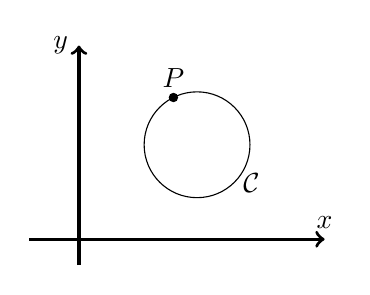
\begin{tikzpicture}[scale=0.3]

\draw[very thick, ->] (-2.1,0) -- (10.4,0) node[above] {$x$};
\draw[very thick, ->] (0,-1.1) -- (0,8.2) node[left] {$y$};

\draw (5, 4) circle (2.24);
\node at (7.3, 2.4) {$\mathcal{C}$};
\fill (4, 6) circle (0.2) node[above] {$P$};

\end{tikzpicture}
\end{minipage}

\begin{questions}
\vspace{-10mm}
\question[2] Show that $P(4, 6)$ lies on $\mathcal{C}$.

\vspace{5mm}
LHS = \makebox[140mm]{\dotfill} \\

\vspace{0mm}
RHS = \makebox[140mm]{\dotfill}

\fullwidth{Define the object $m : 2y = x + 8$.}
\question[2] What is the nature of $m$, and explain how you can tell. \hfill \emph{(line, circle, point, \ldots)}
\fillwithdottedlines{15mm}

\question[2] Show that $P \in m$.
\fillwithdottedlines{25mm}

\question[2] Determine the gradient and $y$-intercept of $m$.
\fillwithdottedlines{25mm}

\question[2] What is the center and radius of $\mathcal{C}$?
\fillwithdottedlines{\stretch{1}}

\question \textbf{Bonus.} Show that $m$ is tangent to $\mathcal{C}$. \hfill \emph{Work overleaf.}

\end{questions}

\begin{tcolorbox}

\textbf{Name of marker:}

\begin{center}
\gradetable[h][questions]
\end{center}

\end{tcolorbox}


\end{document}